%
%   This file is part of the APS files in the REVTeX 4.1 distribution.
%   Version 4.1r of REVTeX, August 2010
%
%   Copyright (c) 2009, 2010 The American Physical Society.
%
%   See the REVTeX 4 README file for restrictions and more information.
%
% TeX'ing this file requires that you have AMS-LaTeX 2.0 installed
% as well as the rest of the prerequisites for REVTeX 4.1
%
% See the REVTeX 4 README file
% It also requires running BibTeX. The commands are as follows:
%
%  1)  latex apssamp.tex
%  2)  bibtex apssamp
%  3)  latex apssamp.tex
%  4)  latex apssamp.tex
%
\documentclass[%
 reprint,
%superscriptaddress,
%groupedaddress,
%unsortedaddress,
%runinaddress,
%frontmatterverbose, 
%preprint,
%showpacs,preprintnumbers,
%nofootinbib,
%nobibnotes,
%bibnotes,
 amsmath,amssymb,
 aps,
%pra,
%prb,
%rmp,
%prstab,
%prstper,
%floatfix,
]{revtex4-1}

\usepackage{graphicx}% Include figure files
\usepackage{dcolumn}% Align table columns on decimal point
\usepackage{bm}% bold math
\usepackage{mathtools}
\graphicspath{ {pics/} }
%\usepackage[mathlines]{lineno}% Enable numbering of text and display math
%\linenumbers\relax % Commence numbering lines

%\usepackage[showframe,%Uncomment any one of the following lines to test 
%%scale=0.7, marginratio={1:1, 2:3}, ignoreall,% default settings
%%text={7in,10in},centering,
%%margin=1.5in,
%%total={6.5in,8.75in}, top=1.2in, left=0.9in, includefoot,
%%height=10in,a5paper,hmargin={3cm,0.8in},
%]{geometry}

\begin{document}

\title{College Scorecard}% Force line breaks with \\
\thanks{Intended to accompany the Exploratory Data Analysis Presentation.}%

\author{Caleb Dowdy}
\author{Nicole Navarro}
\author{Lance Price}
\author{Eric Voorhis}


\begin{abstract}
	Is there a significant difference in cost and earnings for the three different school types (Public, Private Non-profit, and Private for-profit) present in the College Scorecard data? In order to measure and quantify these differences a discussion of completeness and model suitability is required. Completeness of the college scorecard data set is assessed in order provide a hard limit on the utility of said data set and how that impacts the overall reliability of the conclusions drawn. Our statistical analysis consisted of an analysis of variance(ANOVA) and a multiple linear regression model(MLR). Both ANOVA and MLR require that certain assumptions are met in order to guarantee the credibility of the results. The results of our linear modeling indicate that further efforts must be made in order capture diminishing marginal returns of cost in our earnings function and that our earnings function was missing a variable accounting for the talent of the student body.
\end{abstract}

\maketitle
%\tableofcontents

\section{\label{sec:level1}Introduction}
Picking the right school is a very important choice to make.  The government has good reason to help students and parents make more informed choices about where students should go to college.  It helps the government because there will probably be more productive members of society if they make better choices about their education.  These better choices could lead to more positive outcomes of debt repayment, more money cycling through the economic machine, and more taxes being paid to the government.  In addition, having more information about colleges can help the government make better choices about which colleges they should invest more money into.  All of these motivations are centered around which colleges are most valuable to the individual students and to the government as a whole.  This begs the question: how do we define how valuable a college is?  One possible definition involves some combination of future earnings and total cost of education.

\section{\label{sec:level1}Variables of Interest and Statement of Thesis}
These motivations inspired us to look at certain variables in the College Scorecard dataset.  The general variables of interest are earnings and cost.  The specific variables in the dataset that we focused our attention on are total cost of attendance and median earnings of un-enrolled students 10 years after their first reported enrollment date.  We were curious to see whether there were significant differences in these two variables between different school types, so we also looked at the variable named control.  The variable categorizes all schools by whether they are public, private for-profit, or private nonprofit. Our thesis statement focuses on these variables: \textit{ Is there a significant difference in cost and earnings for these three types of school?}  After identifying our variables of interest and thesis statement, we must look at these variables in more detail.


\section{\label{sec:level1}Completeness}
Here will be a discussion of how complete the college scorecard is.Breakdown of individual characteristic... etc. 

\section{\label{sec:level1}Analysis}
Our analysis of the differences between the types of schools present in the college scorecard dataset consisted of linear modeling; specifically ANOVA and Multiple Linear Regression.  These models will be discussed separately in the following subsections. 

\subsection{\label{sec:level2}ANOVA}
A natural way to analyze the difference among group means is through the use of ANOVA.  Several assumptions must be observed in order to correctly perform an ANOVA.  Violating any one of these given assumption could result in overestimation and false positives.  One of these assumptions requires that variables of interest are normally distributed.  When we looked at the density plots of the distributions of median earnings for the three school types, the public and private nonprofit school distributions were close to normal distributions (Figure 1).  The distribution of median earnings for private for-profit institutions (pink distribution) showed an obvious bimodal distribution.  Thus, we only went forward in the ANOVA for the public and private nonprofit schools.  The following table shows the results of the ANOVA.

% Mon Nov  7 16:25:58 2016
\begin{table}[ht]
	\centering
	\caption{Summary of ANOVA for Earnings on Public and Private Nonprofit Institutions}
	\begin{tabular}{lrrrrr}
		  \hline
		   & Df & Sum Sq & Mean Sq & F value & Pr($>$F) \\ 
		     \hline
		     Control & 1 & 1.4E11 & 1.4E11 & 835.0 & 0.00 \\ 
		       Residuals & 9862 & 1.6E12 & 1.6E8 &  &  \\ 
		          \hline
	\end{tabular}
\end{table}


The table shows that there is a significant difference in the means of median earnings between public and private nonprofit schools, with an F value of 835 (one degree of freedom).  We also looked at the distributions of total cost of attendance for the three school types and concluded that ANOVA would not be a suitable way to study the relationship between cost and school type (Figure 2).  The distributions for the three school types are either multimodal or have heavy tails.  We then moved onto another option for studying the relationship between cost and school type.
\begin{figure}[h]
\caption{Density Plot of Earnings for Different School Type}
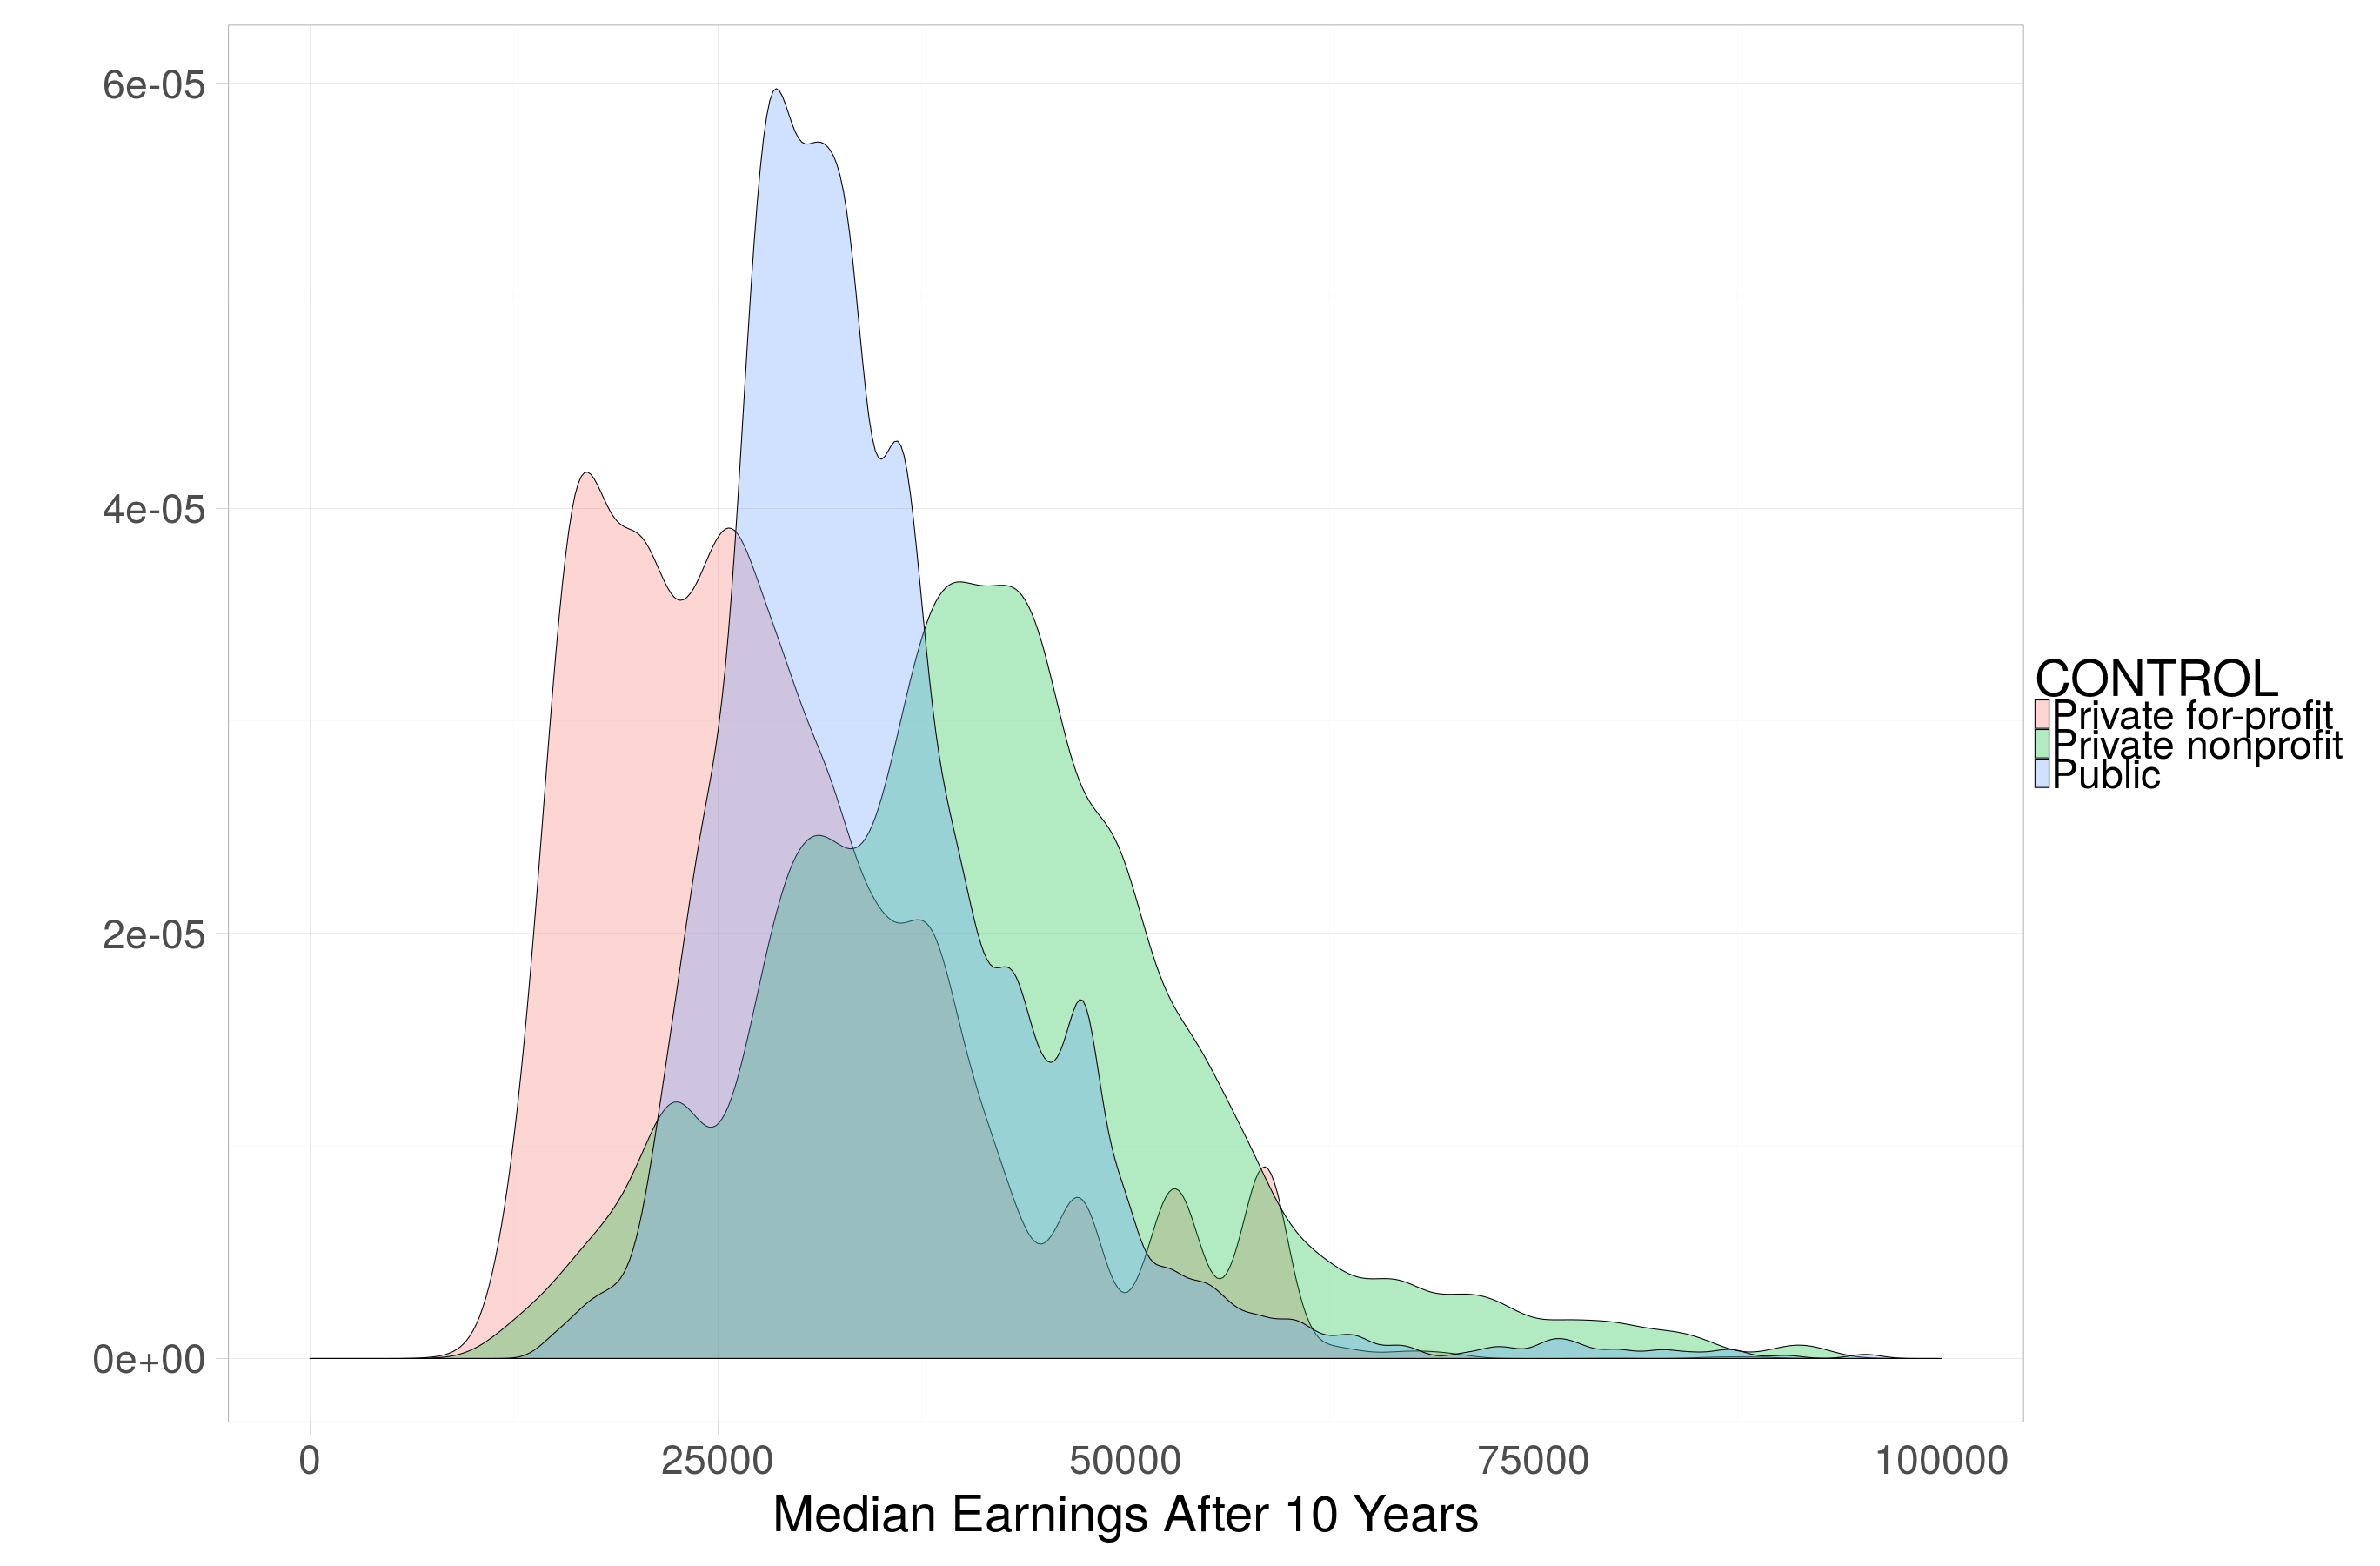
\includegraphics[width=8cm, height=7cm]{earnings.png}
\end{figure}

\begin{figure}[h]
\caption{Density Plot of Cost for Different School Types}
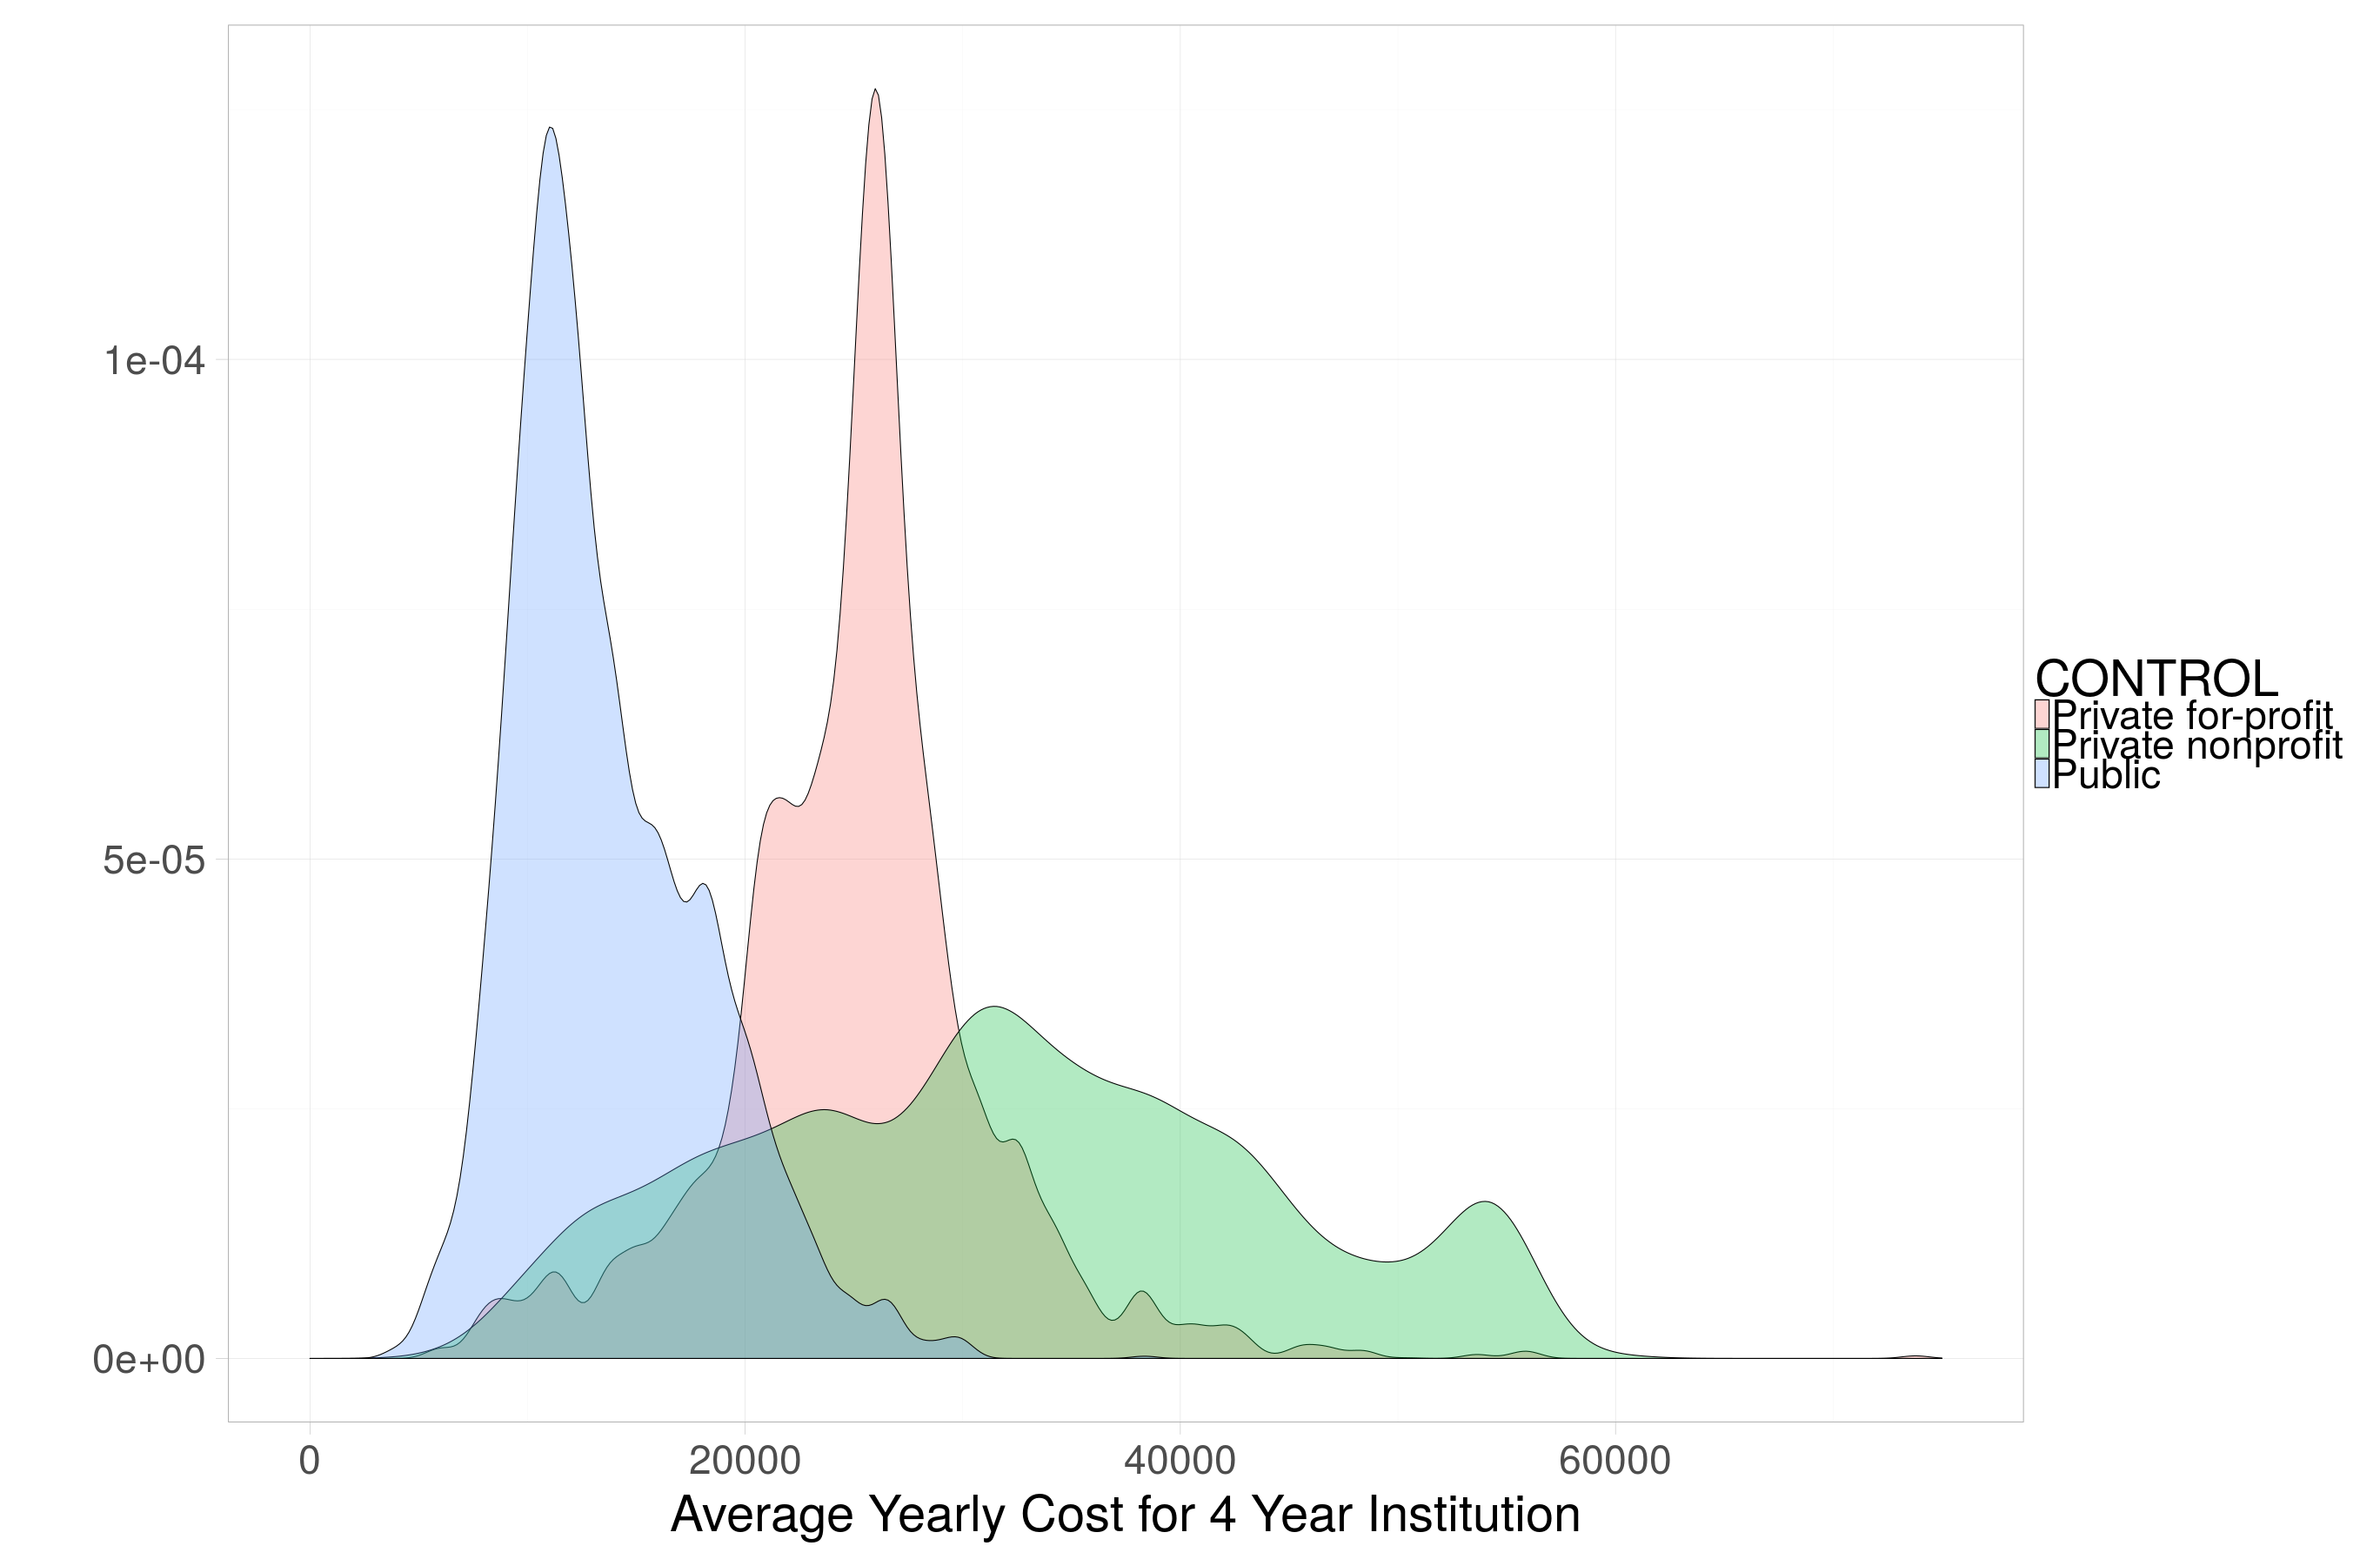
\includegraphics[width=8cm, height=7cm]{cost.png}
\end{figure}

\subsection{\label{sec:level2} Multiple Linear Regression}
The goal of this regression is to quantify the relationship that median earnings (10 years out) has with respect to cost and type of school. Formally stated: 

\begin{align*}
	\mathrm{Earnings} = \beta_{0} 
    &+ \beta_{1}  \mathrm{Cost} + \delta_{2}  \mathrm{Control} + \epsilon\\
\end{align*}

\textbf{Earning} := Median earnings for an institution 10 years after graduation

\textbf{Cost} := Average yearly cost of living and tuition for a 4 year institution.

\textbf{Control} := Factor variable for type of institution; private non-profit, private for-profit, or public.

\vspace{2mm}

The equation shown above can be thought of as a simple linear regression with the inclusion of a factor variable.  Due to the simplicity of this equation it is very limited in it's modeling capabilities. 

% Date and time: Mon, Nov 07, 2016 - 11:20:10 AM
% Requires LaTeX packages: dcolumn 
\begin{table}[!htbp] \centering 
  \caption{Results\footnote{Table created by stargazer v.5.2 by Marek Hlavac, Harvard University. E-mail: hlavac at fas.harvard.edu}} 
  \label{} 
\begin{tabular}{@{\extracolsep{5pt}}lD{.}{.}{-3} } 
\\[-1.8ex]\hline 
\hline \\[-1.8ex] 
 & \multicolumn{1}{c}{\textit{Dependent variable:}} \\ 
\cline{2-2} 
\\[-1.8ex] & \multicolumn{1}{c}{Earnings} \\ 
\hline \\[-1.8ex] 
 Cost & 0.714^{***} \\ 
  & (0.013) \\ 
  & \\ 
 Control: Private nonprofit & 2,661.872^{***} \\ 
  & (289.451) \\ 
  & \\ 
 Control: Public & 9,620.303^{***} \\ 
  & (306.431) \\ 
  & \\ 
 Constant  & 15,103.640^{***} \\ 
  & (398.875) \\ 
  & \\ 
\hline \\[-1.8ex] 
Observations & \multicolumn{1}{c}{7,524} \\ 
R$^{2}$ & \multicolumn{1}{c}{0.342} \\ 
Adjusted R$^{2}$ & \multicolumn{1}{c}{0.341} \\ 
Residual Std. Error & \multicolumn{1}{c}{8,919.327 (df = 7520)} \\ 
F Statistic & \multicolumn{1}{c}{1,300.003$^{***}$ (df = 3; 7520)} \\ 
\hline 
\hline \\[-1.8ex] 
\textit{Note:}  & \multicolumn{1}{r}{$^{*}$p$<$0.1; $^{**}$p$<$0.05; $^{***}$p$<$0.01} \\ 
\end{tabular} 
\end{table} 

\subsubsection{Results}
The results in Table 2 indicate that 34\% of variation in Earnings are explained by the regression equation. With an F statistic of 1,300.003 we can infer that there is a significant relationship between our independent variables and dependent variable. Coefficients for Cost, Control: Private non-profit, Control: Public, and Constant are all significant at the commonly accepted values of \alpha. 

\subsubsection{Interpretting Cost}
The coefficient on the \textit{Cost} term implies that for a \$1 increase in yearly average cost would amount to a \$.71 increase in median earnings 10 years after graduation. Intuitively a positive coefficient is what we would expect; with costs rising we would expect the quality of education to increase and the cost of living to increase, ceterus parabus. Assuming that increasing costs can be used as a proxy for the quality of education is a strong assumption, instead we expand to include the cost of living as well. When tuition and cost of living go up, we would expect earnings to follow. Our model suggests that a student at a four year institution can expect \$.71 on the dollar spent towards cost of living and tuition, ceterus parabus. 

\subsubsection{Interpretting Control}
The coefficients of Control: Private nonprofit and Control: Public are measured relative to the missing category (Control: for-profit).  Control: Private non-profit has a positive coefficient of 2,661.87 which can be interpreted as the increase in median earnings 10 years after graduation by attending a private non-profit over a private for-profit.  Similarly, the coefficient of 9,620.30 can be interpreted as the increase in median earnings 10 years after graduation by attending a public institution over a private for-profit institution.


\subsubsection{Recomendations and Further Research}
If a students main priority is to maximize their earning potential 10 years after graduation, our model would suggest that they should consider attending a public school and spend as much as possible. For obvious reasons this cannot be the case, there must exist a point at which earnings experiences diminishing marginal returns with respect to cost. We recommend that in further analysis we include a quadratic cost term in order to test our hypothesis regarding diminishing marginal returns. Our model explained roughly 34\% of variation in Earnings which leads us to believe that there are lurking variable which could increase our explanatory power.  Currently, our model lacks any kind of proxy for the talent present at a given university.  A substantial amount of literature suggests a significant positive relationship between an individuals earnings and their IQ. Using a variable for median/mean SAT scores for a given institution would serve as a good proxy for IQ and hopefully increase the overall explanatory power.  

\section{\label{sec:level1}Conclusions}
After accessing completeness of the data and performing the above analysis, we came to a few conclusions.  The first and most jarring conclusion was that the data is very sparse for many of the variables of interest to us.  The second main conclusion was that the ANOVA showed a significant difference in median earnings for public and private nonprofit schools.  The third main conclusion was that a linear model showed a possible relationship between cost, earnings, and school type.

Future areas to concentrate on would be incorporating average SAT scores into the linear model and calculating the NPV (Net Present Value) of going to each school.  This would both help to illuminate what makes a school more valuable to students, the government, and society as a whole.


\end{document}
%
% ****** End of file apssamp.tex ******
